%!TEX root = ../Project.tex
\section{Introduction} 
\label{introduction}
       
A RPG (Role Playing Game) is game where player assumes the role of on the character. A RPG is usually story driven and the character usually has quest to complete. In the course of the game the player will go to different environments such as town and dungeons. In they these environments the player will have to battle opponents in battles. Combat in RPGs is normally a simple turn based system where player and the opponents take turns attacks each other using various skills. 

A Tactical RPG is sub-genre of an RPG that focuses on the combat side of the genre. A Tactical RPG is series of \texttt{battles}, which take place in various environments intertwined with an over-aching story.

Each \texttt{battle} is grid based (like chess) where each player has a number of units(pieces). 
\begin{figure}
	[htbp] \centering 
	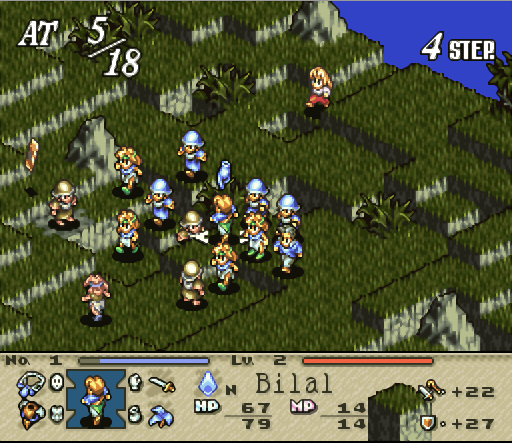
\includegraphics[height=3in]{figures/TRPG.png} \caption{\textbf{Tactics Ogre}\cite{to} a classic Tactical RPG } \label{fig:figures_TRPG} 
\end{figure}
The players taken turns to moves their units. Each unit has attributes associated with it such as strength, and hit points that affect all the actions in the game. Like chess there are different kinds of units which affects how the unit moves and what action they can perform. A unit can attack other player's units, the goal of the battle is usually to defeat all the opponents units.

The aim of this project is to create a engine which will take resources such as graphics, sound and rules of the game to create a runnable Tactical RPG.